\documentclass[11pt]{beamer}

\usepackage{amsmath}
\usepackage{amssymb}
\usepackage{graphicx}
\usepackage{caption}
\usepackage{subcaption}
\usepackage{multirow}
\usepackage{placeins}

\graphicspath{{images/}}

\let\bld\boldsymbol

\bibliographystyle{plain}

\title{{\large MATH 579 Numerical PDEs} \vspace{0.2in} \\ Discontinuous Galerkin method with \\ Taylor basis functions}
\author{Aditya Kashi}
\date{April 25, 2017}

\AtBeginSection{
	\begin{frame}{Table of Contents}
		\tableofcontents[currentsection]
	\end{frame}
}

\begin{document}

\begin{frame}
\maketitle
\end{frame}

\section{Introduction}
\begin{frame}{Introduction}
Nodal Lagrange finite elements are by far the most commonly used as the polynomial basis of choice.
\vspace{0.2in}

However, an alternative exists in modal basis functions, such as Legendre basis and Taylor basis.
\end{frame}

\begin{frame}{Why Taylor basis?}
Some advantages that the modal Taylor basis functions over nodal Lagrange basis functions \cite{luo_taylor, aizinger_scaleseparation}:
\begin{itemize}
\item \emph{Hierarchical}. Easier implementation of p-adaptation  and p-multigrid solvers.
\item Remains same irrespective of the geometric type of elements. This makes for easier implementation of codes. Another aspect is that number of DOFs is less than that in case of nodal basis for non-simplicial elements, while maintaining optimal order of accuracy (hopefully)
\item Implementation of reconstruction DG methods becomes efficient and elegant. Reconstruction DG: increase accuracy without increase in number of DOFs, using high-order finite volume ideas.
\end{itemize}
\end{frame}

\section{Governing equations}
\begin{frame}
A hyperbolic partial differential equation in $n_d$ spatial dimensions can be written as
\begin{equation}
\frac{\partial \bld{u}}{\partial t} + \sum_{j=1}^{n_d} \frac{\partial \bld{F}_j}{\partial x_j} = \bld{0} \quad \bld{x} \in \Omega, t \in [0,T]
\label{conservativeGE}
\end{equation}
with some initial condition
\begin{equation}
\bld{u}(\bld{x},0) = \bld{u}_0(\bld{x})
\end{equation}
and some combination of several possible types of boundary conditions.
\end{frame}
\begin{frame}
Here, we consider the steady 2-dimensional linear advection equation.
\begin{equation}
\nabla\cdot(\bld{\beta}u) = f, \quad \bld{x} \in [-\frac32,\frac32]\times[-1,1]
\end{equation}
where $f(x,y) = \frac{2\pi}{3}\cos\frac{2\pi}{3}(x+\frac32)$, $\bld{\beta} = (1,0)$.

True solution: $u(x,y) = \sin\frac{2\pi}{3}(x+\frac32)$

We solved it here by iterating in `pseudo-time' to steady state using explicit time-stepping.
\begin{equation}
\frac{\partial u}{\partial \tau} + \nabla\cdot(\bld{\beta}u) = f
\end{equation}
\end{frame}

\section{Finite element formulation}

\begin{frame}
The discrete function space for some positive integer $k$
\begin{align}
W_{K} &:= \mathbb{P}_k(K), \quad K \in \mathcal{T}_h \\
W_h &:= \bigoplus_{K \in \mathcal{T}_h} W_{K}
\end{align}
$\bigoplus$ denotes a direct sum \cite{nodaldg}.

Discrete weak formulation on each element: Find $u_h \in W_{K}$ such that
\begin{equation}
\int_{K} \frac{\partial u_h}{\partial t}w\,d\mu + \int_{\partial K} \bld{F}(u_h)\cdot\hat{\bld{n}}w \,ds - \int_{K}\bld{F}(u_h)\cdot\nabla w \,d\mu = \bld{0} 
\label{wf}
\end{equation}
$ \forall w \in W_{K},\, K \in \mathcal{T}_h$.
\end{frame}
\begin{frame}
Introducing basis functions and numerical flux, the discrete form becomes: find the $n$ DOFs $u_j$ of each conserved variable $\mathbf{u} \in \mathbb{R}^n$, such that
\begin{multline}
\sum_{j=1}^n\int_{K} b_ib_j\,d\mu\, \frac{d\mathbf{u}}{d t} + \int_{\partial K}  h(\bld{u}_L(\bld{x}), \bld{u}_R(\bld{x}), \hat{\bld{n}})b_i \,ds \\ -\int_{K}\bld{F}(u_h(\bld{x}))\cdot\nabla b_i \,d\mu = \bld{0}, \quad i \in {1,...n},\, K \in \mathcal{T}_h.
\label{df}
\end{multline}
\end{frame}

\section{Taylor basis functions}
\begin{frame}{Taylor series}
In a Taylor basis, a function is expressed as a Taylor expansion about the element center. In 2D, a quadratic or P2 expansion in an element e would be written as
\begin{multline}
u_h = u_c + \frac{\partial u}{\partial x} \Big|_c(x-x_c) + \frac{\partial u}{\partial y} \Big|_c(y-y_c) \\ + \frac{\partial^2 u}{\partial x^2} \Big|_c \frac{(x-x_c)^2}{2} + \frac{\partial^2 u}{\partial y^2} \Big|_c \frac{(y-y_c)^2}{2} + \frac{\partial^2 u}{\partial x\partial y} \Big|_c (x-x_c)(y-y_c)
\label{eqn:taylorexpn_orig}
\end{multline}
\end{frame} 
\begin{frame}
We can take an average of both sides over the element to get
\begin{multline}
\tilde{u} = u_c + \frac{\partial u}{\partial x} \Big|_c \frac{1}{|K|}\int_K(x-x_c)d\mu + \frac{\partial u}{\partial y} \Big|_c \frac{1}{|K|}\int_K (y-y_c)d\mu \\ \, + \frac{\partial^2 u}{\partial x^2} \Big|_c \frac{1}{|K|}\int_K \frac{(x-x_c)^2}{2}d\mu + \frac{\partial^2 u}{\partial y^2} \Big|_c \frac{1}{|K|}\int_K \frac{(y-y_c)^2}{2}d\mu \\ + \frac{\partial^2 u}{\partial x\partial y} \Big|_c \frac{1}{|K|}\int_K (x-x_c)(y-y_c)d\mu \\
= u_c + \frac{\partial^2 u}{\partial x^2} \Big|_c \frac{1}{|K|}\int_K \frac{(x-x_c)^2}{2}d\mu + \frac{\partial^2 u}{\partial y^2} \Big|_c \frac{1}{|K|}\int_K \frac{(y-y_c)^2}{2}d\mu \\+ \frac{\partial^2 u}{\partial x\partial y} \Big|_c \frac{1}{|K|}\int_K (x-x_c)(y-y_c)d\mu
\end{multline}
\end{frame}
\begin{frame} 
This last equation can be subtracted from \eqref{eqn:taylorexpn_orig} to get
\begin{multline}
u_h = \tilde{u} + \frac{\partial u}{\partial x} \Big|_c(x-x_c) + \frac{\partial u}{\partial y} \Big|_c(y-y_c) \\+ \frac{\partial^2 u}{\partial x^2} \Big|_c \left( \frac{(x-x_c)^2}{2} - \frac{1}{|K|}\int_K \frac{(x-x_c)^2}{2}d\mu \right) \\ + \frac{\partial^2 u}{\partial y^2} \Big|_c \left( \frac{(y-y_c)^2}{2} -\frac{1}{|K|}\int_K \frac{(y-y_c)^2}{2}d\mu \right) \\+ \frac{\partial^2 u}{\partial x\partial y} \Big|_c \left( (x-x_c)(y-y_c) - \frac{1}{|K|}\int_K (x-x_x)(y-y_x)d\mu \right).
\label{eqn:taylorexpn}
\end{multline}
\end{frame}
\begin{frame}{Taylor Basis Functions}
\begin{align}
&B_1(\bld{x}) = 1 \\
&B_2(\bld{x}) = \frac{(x-x_c)}{\Delta x} \\
&B_3(\bld{x}) = \frac{(y-y_c)}{\Delta y} \\
&B_4(\bld{x}) = \left( \frac{(x-x_c)^2}{2\Delta x^2} - \frac{1}{|K|}\int_K \frac{(x-x_c)^2}{2}d\mu \right) \\
&B_5(\bld{x}) = \left( \frac{(y-y_c)^2}{2\Delta y^2} -\frac{1}{|K|}\int_K \frac{(y-y_c)^2}{2}d\mu \right) \\
&B_6(\bld{x}) = \left( \frac{(x-x_c)(y-y_c)}{\Delta x\Delta y} - \frac{1}{|K|}\int_K (x-x_c)(y-y_c)d\mu \right)
\end{align}
\end{frame}
\begin{frame}{Degrees of Freedom}
\begin{align}
L_1(u) := \tilde{u} \\
L_2(u) := \frac{\partial u}{\partial x}\Big|_c \Delta x \\
L_3(u) := \frac{\partial u}{\partial y}\Big|_c \Delta y \\
L_4(u) := \frac{\partial^2 u}{\partial x^2}\Big|_c 2\Delta x^2 \\
L_5(u) := \frac{\partial^2 u}{\partial y^2}\Big|_c 2\Delta y^2 \\
L_6(u) := \frac{\partial^2 u}{\partial x\partial y}\Big|_c \Delta x\Delta y
\end{align}
$\Delta x$ and $\Delta y$ are $\frac12 (x_{max}-x_{min})$ and $\frac12 (y_{max}-y_{min})$ respectively.
\end{frame}

\begin{frame}{The `Taylor finite element'}
Ciarlet: A finite element is a triplet $(K, P_K, \Sigma_K)$ where 
\begin{itemize}
\item $K$ is a compact connected Lipschitz subset of $\mathbb{R}^n$ with nonempty interior, 
\item $P_K$ is a finite dimensional vector space of functions $K \rightarrow \mathbb{R}^p$, $p \in \mathbb{N}$ and 
\item $\Sigma_K$ is a finite set of linear functionals $P_K \rightarrow \mathbb{R}$ called the local degrees of freedom.
\end{itemize}

Local degrees of freedom must be \emph{unisolvent}.
\end{frame}

\begin{frame}{\emph{A-priori} error estimate}
Johnson and Pitk\"aranta \cite{johnson_pitkaranta}: the following error estimate holds for $\mathbb{P}_k$ finite elements for scalar linear hyperbolic equations on shape-regular and quasi-uniform meshes:
\begin{equation}
\lVert u-u_h \rVert_{L^2(\Omega)} \leq h^{k+1/2} |u|_{H^{k+1}(\Omega)}.
\end{equation}
\end{frame}

\begin{frame}{Elements defined in physical coordinates}
Taylor basis functions are defined on the physical element, so polynomial functions of these functions or their gradients remain polynomial. 

Terms for mass matrices, stiffness matrices etc. can be integrated exactly by Gaussian quadrature of high-enough order, \emph{even for curved elements} in contrast to Lagrange basis functions, which are defined as \cite{claesjohnson}
\begin{equation}
P_K = \{ p: p(\bld{x}) = \hat{p}(F^{-1}(\bld{x})),\, \bld{x} \in K,\, \hat{p} \in P_{\hat{K}} \}
\end{equation}
For curved elements, $F^{-1}$ is not a polynomial, so integrands will not be polynomials and cannot be integrated exactly.
\end{frame}

\section{Reconstruction DG scheme}
\begin{frame}{DG FEM can be expensive}
Issues with the DG FEM method for any basis: 
\begin{itemize}
	\item High computational cost compared to FV schemes on a given mesh
	\item More expensive than a continuous FEM scheme of the same order on the same grid
\end{itemize}
\end{frame}
\begin{frame}{One solution}
One way of reducing the cost is the reconstruction DG (RDG) FEM scheme \cite{luo_rdg}, based on Taylor basis DG. 
\begin{itemize}
\item High-order accuracy using less degrees of freedom than a DG scheme. 
\item Where the solution is smooth enough, data from neighboring elements can be used to `reconstruct' a higher-order solution. 
\item Reconstruction in the strong sense.
\item Popular in finite volume community for gradient reconstruction in 2nd order schemes.
\end{itemize}
\end{frame}
\begin{frame}{Reconstruction of 2nd derivatives}
Consider a DG P1 scheme with Taylor elements. Suppose $u \in C^2$ in a neighborhood of element $i$. Write $u(x)$ as a Taylor series on the von-Neumann neighborhood
\begin{multline}
u(\bld{x}) \approx \tilde{U}_i + U_{xi}B_{i_2}(\bld{x}) + U_{yi}B_{i_3}(\bld{x}) \\+ U_{xxi} B_{i_4}(\bld{x}) + U_{yyi} B_{i_5}(\bld{x}) + U_{xyi} B_{i_6}(\bld{x})
\end{multline}
\end{frame}
\begin{frame}
The above function and its derivatives can be evaluated at the element-centres $\bld{x}_j$ of each of the face-neighbouring elements $j$.
\begin{multline}
u_j = \tilde{U}_i + U_{xi}B_{i_2}(\bld{x}_j) + U_{yi}B_{i_3}(\bld{x}_j) \\+ U_{xxi} B_{i_4}(\bld{x}_j) + U_{yyi} B_{i_5}(\bld{x}_j) + U_{xyi} B_{i_6}(\bld{x}_j) \\
\frac{\partial u}{\partial x}\Big|_j = U_{xi}/\Delta x_i + U_{xxi} B_{i_2}(\bld{x}_j) / \Delta x_i + U_{xyi} B_{i_3}(\bld{x}_j) /\Delta x_i \\
\frac{\partial u}{\partial y}\Big|_j = U_{yi}/\Delta y_i + U_{xyi} B_{i_2}(\bld{x}_j) / \Delta y_i + U_{yyi}B_{i_3}(\bld{x}_j)/\Delta y_i
\end{multline}
\end{frame}
\begin{frame}{Least-squares reconstruction}
Arrange into the following system for each neighbor $j$.
\begin{equation}
\begin{bmatrix}
B_4^j & B_5^j & B_6^j \\
0 & B_2^j & B_3^j \\
0 & B_2^j & B_3^j
\end{bmatrix}
\begin{bmatrix}
U_{xxi} \\ U_{xyi} \\ U_{yyi}
\end{bmatrix} =
\begin{bmatrix}
u_j - (\tilde{U}_i + U_{xi}B_2^j + U_{yi}B_3^j) \\
\frac{\Delta x_i}{\Delta x_j}U_{xj} - U_{xi} \\
\frac{\Delta y_i}{\Delta y_j}U_{yj} - U_{yi}
\end{bmatrix} =:
\begin{bmatrix}
R_1^j \\ R_2^j \\ R_3^j
\end{bmatrix}
\end{equation}
Stack all of them to get 12x3 system for quads or 9x3 system for triangles. Solve in least-squares sense.

Implementation: normal equations. Pre-invert the left hand side.
\end{frame}

\section{Results}
\begin{frame}{Mesh}
\begin{figure}
	\centering
	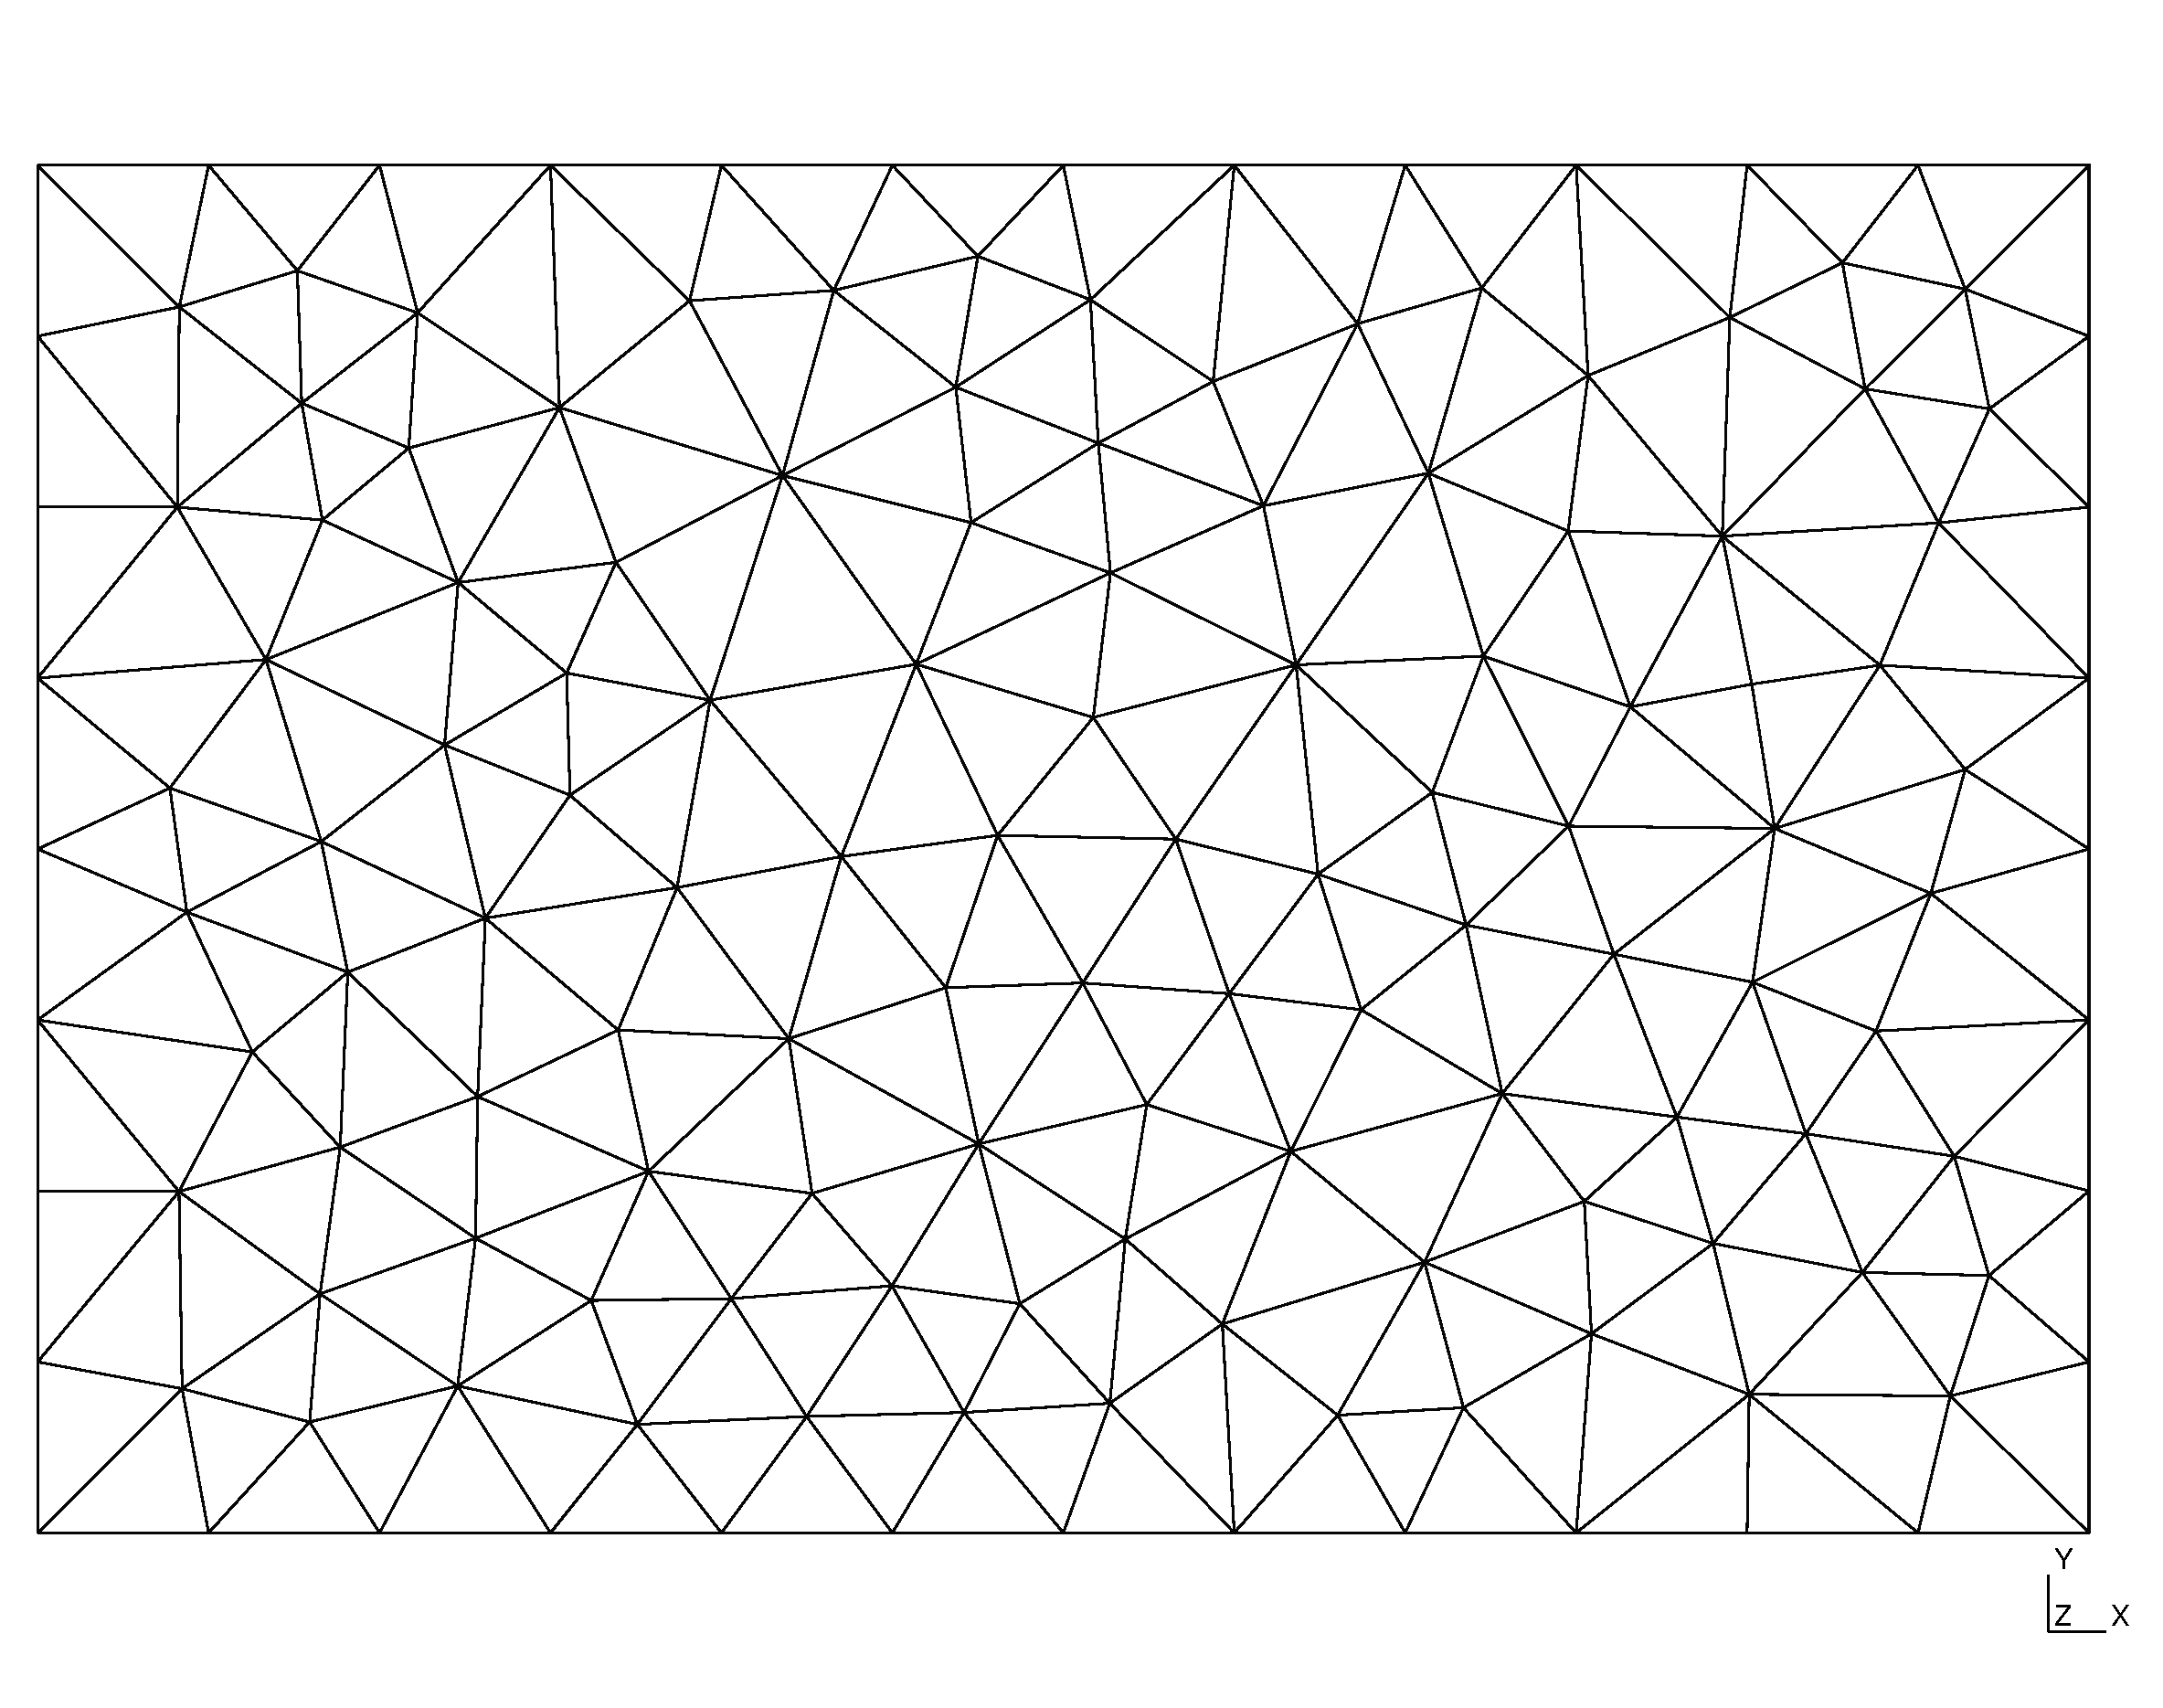
\includegraphics[scale=0.25]{meshtri}
	\caption{One of the triangular meshes used}
\end{figure}
\end{frame}
\begin{frame}{Mesh}
\begin{figure}
	\centering
	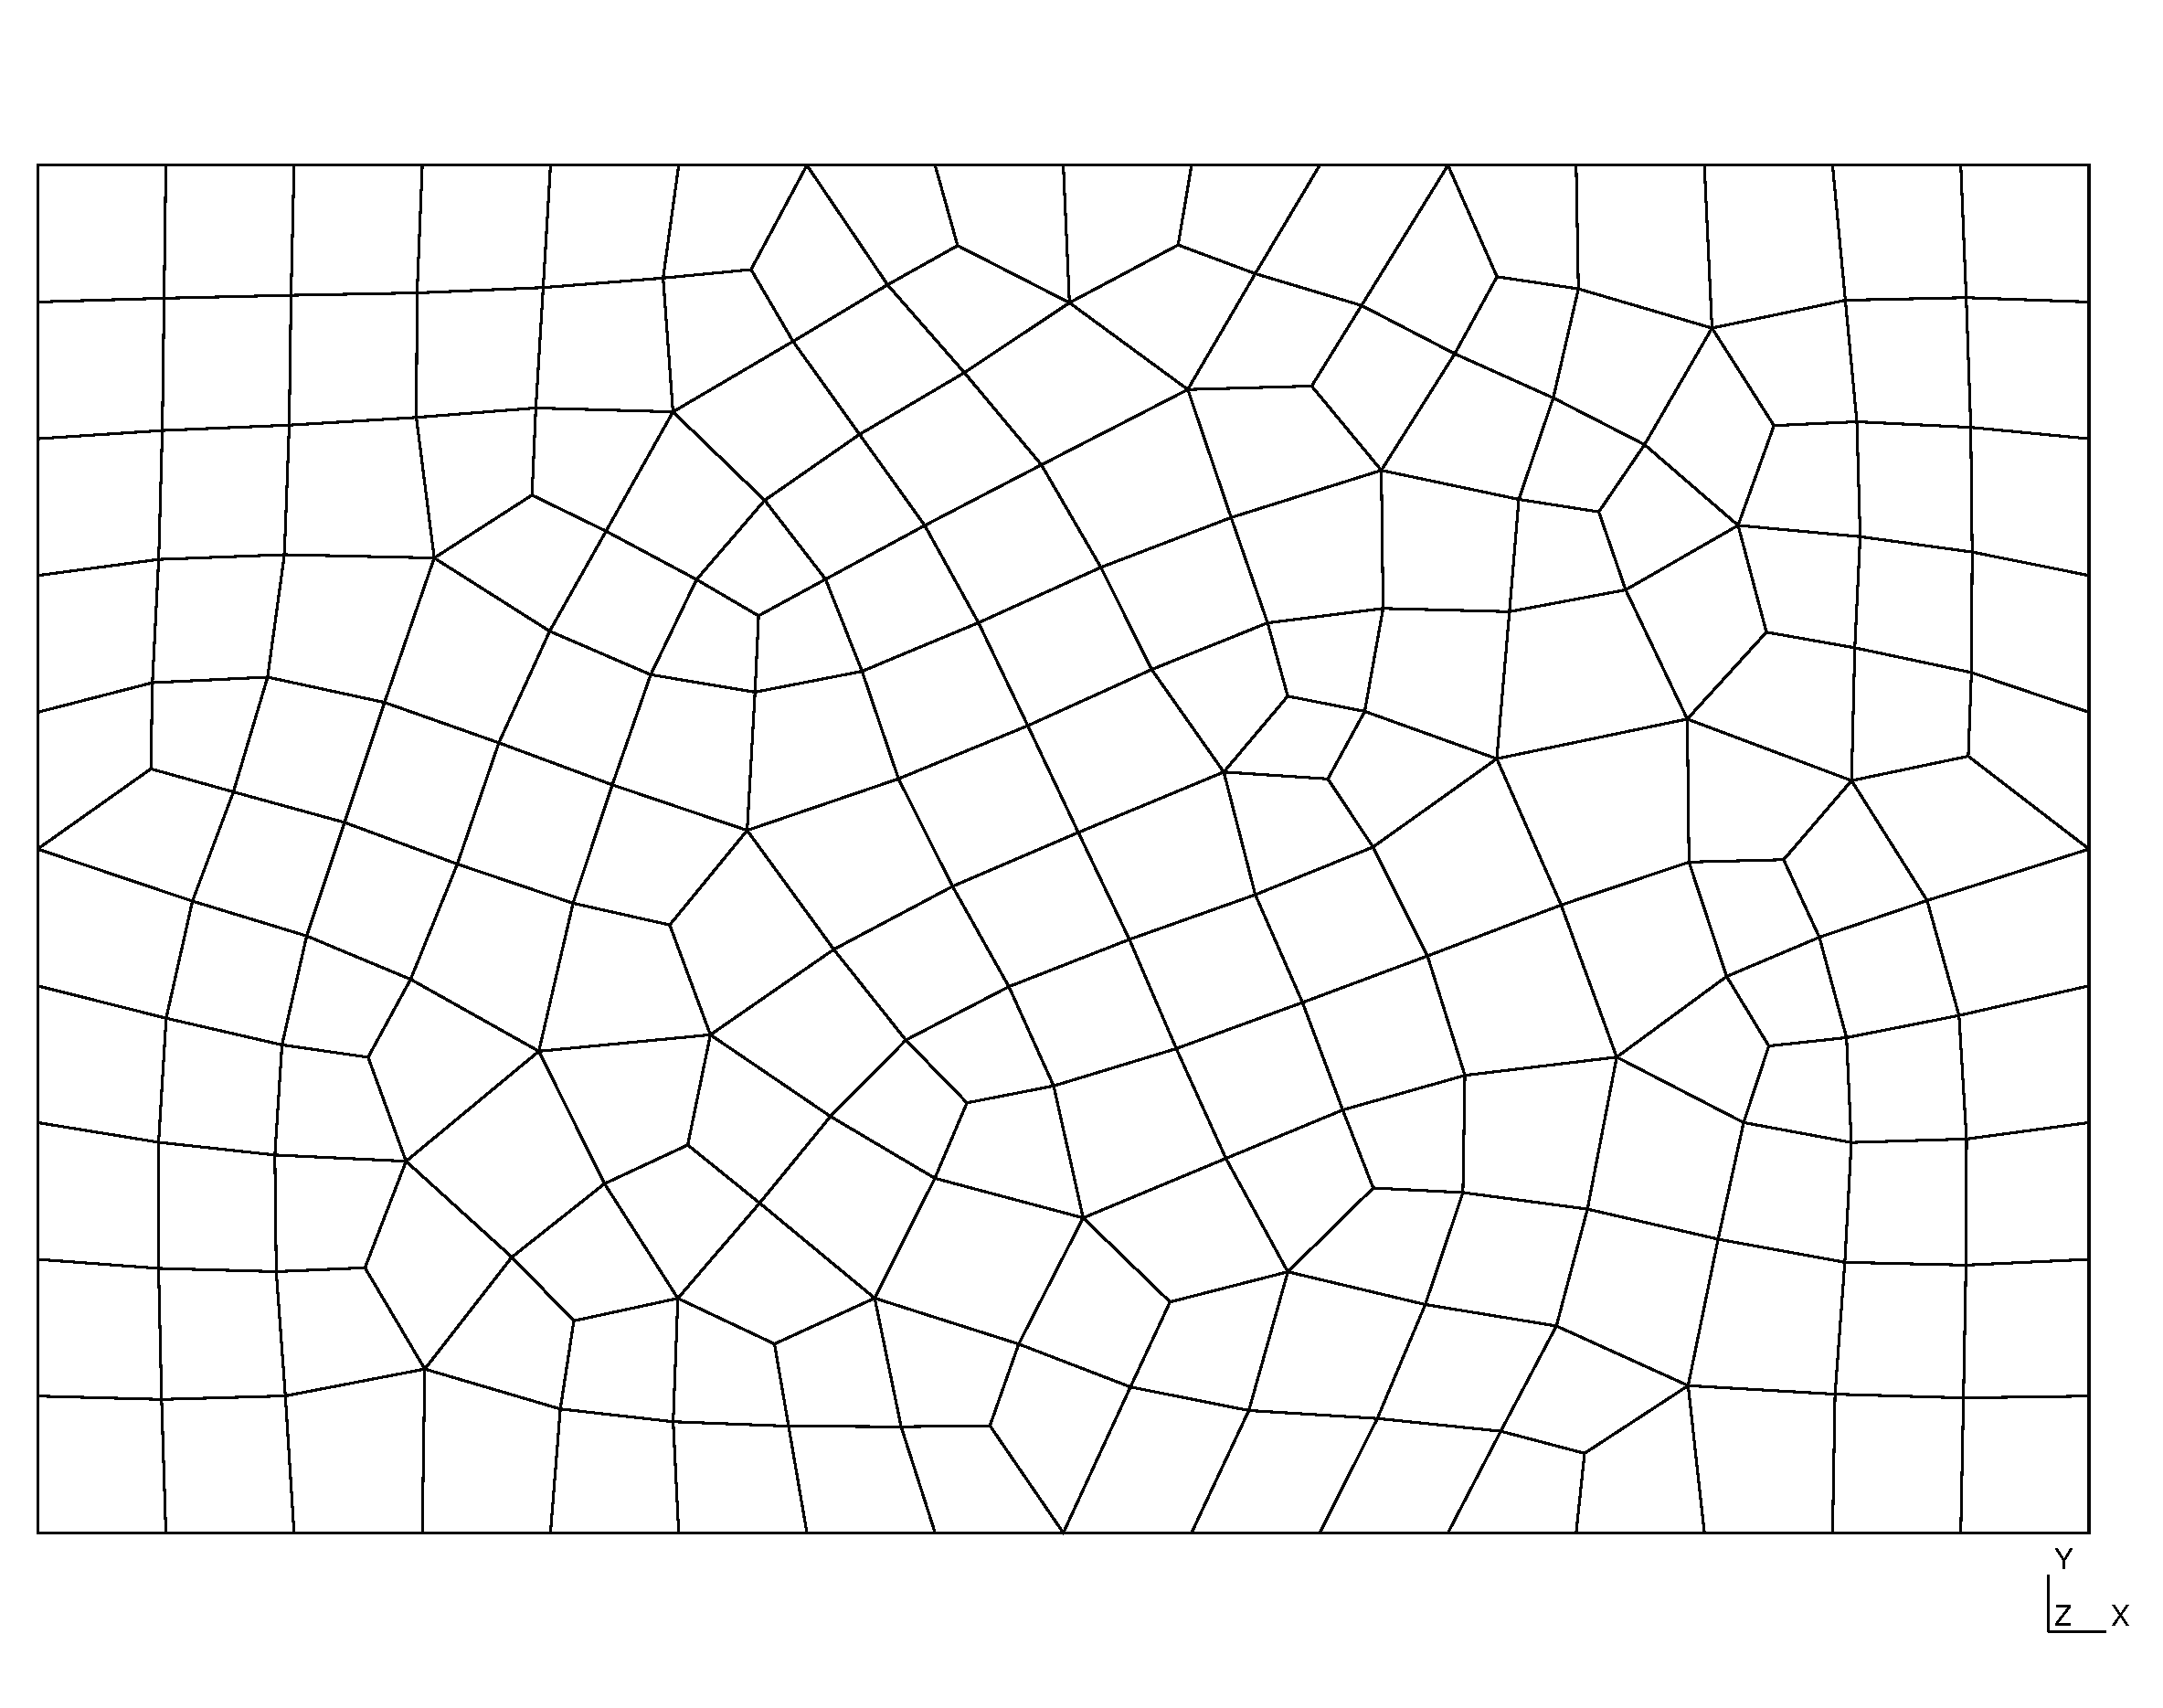
\includegraphics[scale=0.25]{meshquad}
	\caption{One of the quadrangular meshes used}
\end{figure}
\end{frame}
\begin{frame}{Solution}
\begin{figure}
	\centering
	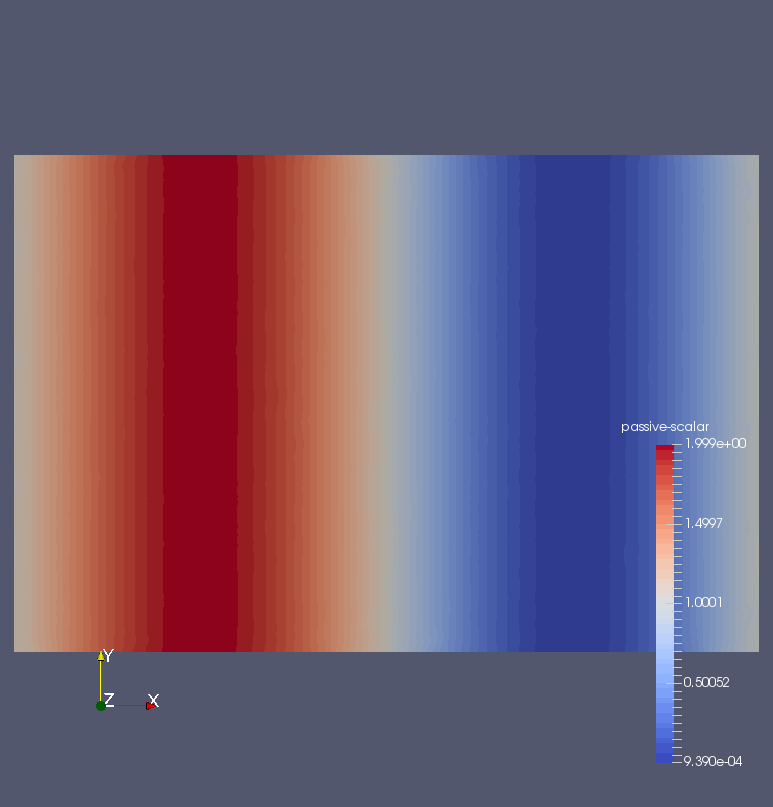
\includegraphics[scale=0.25]{solution-steady-linadv}
	\caption{Sinusoidal in x-direction}
\end{figure}
\end{frame}
\begin{frame}{Convergence: P1}
\begin{figure}
	\centering
	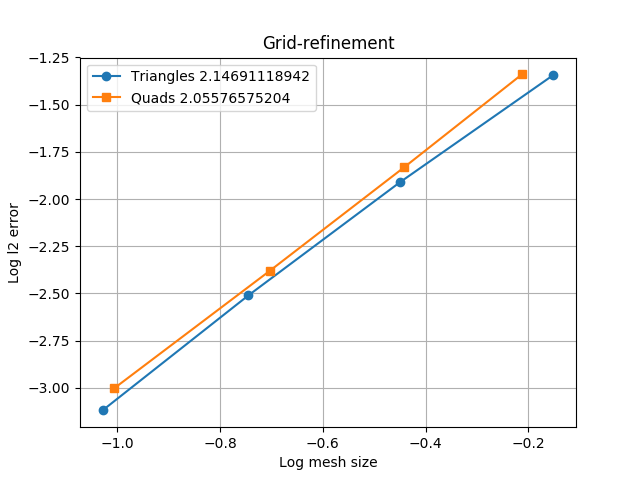
\includegraphics[scale=0.5]{linadv-taylor-p1}
	\caption{Convergence w.r.t. mesh size parameter $h$ for P1}
\end{figure}
\end{frame}
\begin{frame}{Convergence: P2}
\begin{figure}
	\centering
	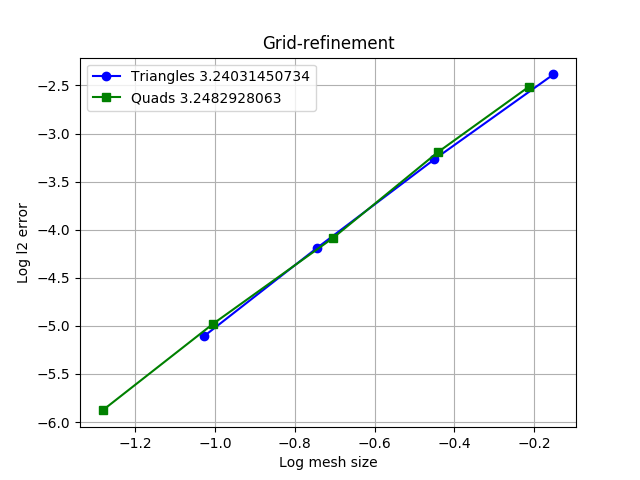
\includegraphics[scale=0.5]{linadv-taylor-p2}
	\caption{Convergence w.r.t. mesh size parameter $h$ for P2}
\end{figure}
\end{frame}
\begin{frame}{Convergence: P2}
\begin{figure}
	\centering
	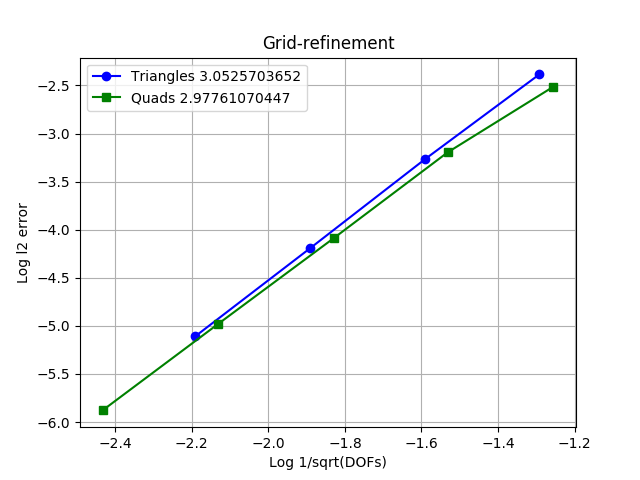
\includegraphics[scale=0.5]{linadv-taylor-p2-dofs}
	\caption{Convergence w.r.t. $\sqrt N_{dof}$ for P2}
\end{figure}
\end{frame}

\section{Conclusions}
\begin{frame}{Limitations of Taylor Elements}
\begin{itemize}
	\item Defined in physical space, basis functions need to stored for each element.
	\item In implicit schemes, element blocks will be dense; might be practically limited to `moderately' high-order for industry-scale problems.
	\item Reconstruction makes the stencil non-compact! Maybe reconstruction can be ignored in Jacobians for implicit schemes.
\end{itemize}
\end{frame}
\begin{frame}{Advantages of Taylor Elements}
\begin{itemize}
\item Taylor basis functions could provide a viable alternative to Lagrange basis functions for simulations of hyperbolic problems; easier to implement!
\item \emph{p}-multigrid is free; no interpolation needed.
\item Needs further numerical testing and theory but it seems extra DOFs might not be needed for non-simplicial elements.
\item Convenient extension to reconstruction DG to increase accuracy without an increase in the number of DOFs is attractive.
\end{itemize}
\end{frame}

\bibliography{refs}
\end{document}